\pagebreak
\subsubsection{UC3-Modifica account}
\begin{figure}[h] 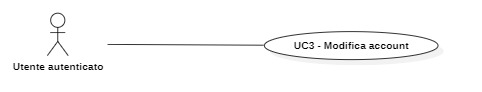
\includegraphics[scale=0.8]{uc03.png} \end{figure}
\begin{itemize}
    \item \textbf{Attore principale:} Utente autenticato;
    \item \textbf{Precondizioni:} L'utente è autenticato all'interno del sistema;
    \item \textbf{Postcondizioni:} Le modifiche fatte alle informazioni dell'account dell'utente sono salvate dal sistema;
    \item \textbf{Scenario principale:}
        \begin{enumerate}
            \item L'utente seleziona l'opzione di modifica dei dati del suo account;
            \item L'utente può inserire:
              \begin{itemize}
                \item La nuova email;
                \item La nuova password con la conferma della nuova password.
              \end{itemize}
            \item L'utente conferma le modifiche fatte;
            \item Il sistema comunica all'utente che la modifica è avvenuta con successo.
        \end{enumerate}
\end{itemize}

\subsubsection{UC4-Logout}
\begin{figure}[h] 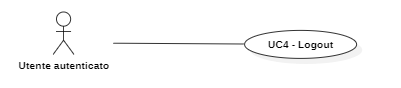
\includegraphics[scale=1]{uc04.png} \end{figure}
\begin{itemize}
    \item \textbf{Attore principale:} Utente autenticato;
    \item \textbf{Precondizioni:} L'utente è autenticato presso il sistema;
    \item \textbf{Postcondizioni:} L'utente non è più autenticato all'interno del sistema;
    \item \textbf{Scenario principale:}
    \begin{enumerate}
        \item L'utente seleziona l'opzione di logout;
        \item Il sistema chiede all'utente la conferma della scelta;
        \item L'utente conferma la scelta;
        \item Il sistema re-indirizza l'utente alla home del sistema.
    \end{enumerate}
\end{itemize}

\pagebreak
\subsubsection{UC5-Creazione profilo}
\begin{figure}[h] 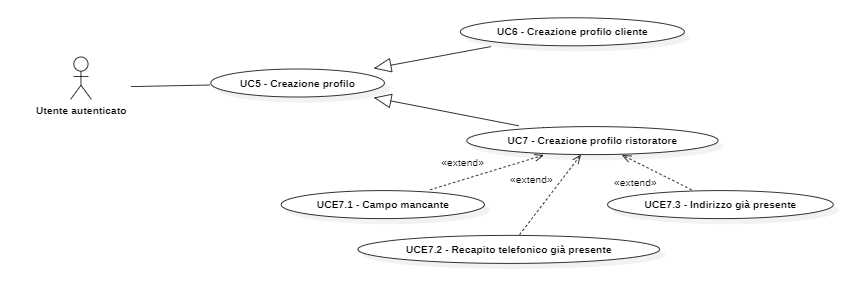
\includegraphics[scale=.7]{uc05.png} \end{figure}
\begin{itemize}
    \item \textbf{Attore principale:} Utente autenticato;
    \item \textbf{Precondizioni:} L'utente è connesso al sistema e sta visualizzando la lista dei suoi profili;
    \item \textbf{Postcondizioni:} Il profilo creato dall'utente, insieme a tutte le relative informazioni, è salvato dal sistema nella lista dei profili dell'utente;
    \item \textbf{Scenario principale:}
    \begin{enumerate}
        \item L'utente seleziona l'opzione di creazione di un nuovo profilo;
        \item Il sistema chiede all'utente di scegliere se creare un profilo di tipo cliente o ristoratore;
        \item L'utente sceglie la tipologia di profilo;
        \item L'utente inserisce i dati necessari per la creazione della tipologia di profilo scelto;
        \item L'utente sceglie l'opzione di conferma dei dati inseriti;
        \item Il sistema comunica all'utente che la creazione del profilo è avvenuta con successo;
        \item L'utente visualizza la lista dei suoi profili, dove è stato aggiunto il profilo appena creato.
    \end{enumerate}
    \item \textbf{Specializzazioni:}
        \begin{itemize}
            \item UC6-Creazione profilo cliente;
            \item UC7-Creazione profilo ristoratore.
        \end{itemize}
\end{itemize}

\subsubsection{UC6-Creazione profilo cliente}
\begin{itemize}
    \item \textbf{Attore principale:} Utente autenticato;
    \item \textbf{Precondizioni:} L'utente è autenticato presso il sistema e sta visualizzando la lista dei suoi profili;
    \item \textbf{Postcondizioni:} Il profilo "cliente" viene salvato dal sistema nella lista dei profili dell'utente;
    \item \textbf{Scenario principale:}
    \begin{enumerate}
        \item L'utente seleziona l'opzione di creazione di un nuovo profilo;
        \item Il sistema chiede all'utente di scegliere se creare un profilo di tipo cliente o ristoratore;
        \item L'utente sceglie la tipologia "cliente";
        \item L'utente inserisce i seguenti dati:
        \begin{itemize}
            \item Il nome;
            \item Il cognome;
            \item Il nome del profilo;
            \item Le eventuali allergie ed intolleranze da una lista precompilata dal sistema.
        \end{itemize}
        \item L'utente sceglie l'opzione di conferma dei dati inseriti;
        \item Il sistema comunica all'utente che la creazione del profilo è avvenuta con successo;
        \item L'utente visualizza la lista dei suoi profili, dove è stato aggiunto il profilo appena creato.
    \end{enumerate}
\end{itemize}

\subsubsection{UC7-Creazione profilo ristoratore}
\begin{itemize}
    \item \textbf{Attore principale:} Utente autenticato;
    \item \textbf{Precondizioni:} L'utente è autenticato presso il sistema e sta visualizzando la lista dei suoi profili;
    \item \textbf{Postcondizioni:} Il profilo-ristoratore appena creato è salvato nella lista dei profili dell'utente;
    \item \textbf{Scenario principale:}
    \begin{enumerate}
        \item L'utente seleziona l'opzione di creazione di un nuovo profilo;
        \item Il sistema chiede all'utente di scegliere se creare un profilo di tipo cliente o ristoratore;
        \item L'utente sceglie la tipologia "ristoratore";
        \item L'utente inserisce i seguenti dati:
        \begin{itemize}
            \item Il nome del ristorante;
            \item L'indirizzo;
            \item Giorni di servizio;
            \item Orari di servizio;
            \item Il recapito telefonico;
            \item Il numero di coperti disponibili;
            \item L'elenco delle tipologie di cucine proposte.
        \end{itemize}
        \item L'utente sceglie l'opzione di conferma dei dati inseriti;
        \item Il sistema comunica all'utente che la creazione del profilo è avvenuta con successo;
        \item L'utente visualizza la lista dei suoi profili, dove è stato aggiunto il profilo appena creato.
    \end{enumerate}
        \item \textbf{Estensioni:}
        \begin{itemize}
                \item UCE7.1-Campo mancante;
                \item UCE7.2-Recapito telefonico già presente;
                \item UCE7.3-Indirizzo già presente.
        \end{itemize}
\end{itemize}

\pagebreak

\textbf{UCE7.1-Campo mancante}
\begin{itemize}
    \item \textbf{Descrizione:} Al momento della conferma dei dati inseriti, nessun campo relativo al ristorante può essere vuoto;
    \item \textbf{Scenario alternativo:}
    \begin{enumerate}
        \item Il sistema verifica che l'utente non abbia inserito i valori relativi ad uno o più campi di compilazione;
        \item Il sistema comunica l'errore all'utente, specificandone la natura;
        \item L'utente visualizza tutti i campi relativi alla creazione del profilo; sono presenti i dati inseriti precedentemente.
    \end{enumerate}
\end{itemize}

\textbf{UCE7.2-Recapito telefonico già presente}
\begin{itemize}
    \item \textbf{Descrizione:} Nel sistema non possono essere presenti ristoranti, afferenti allo stesso ristoratore o a diversi ristoratori, con lo stesso recapito telefonico;
    \item \textbf{Scenario alternativo:}
    \begin{enumerate}
        \item Il sistema rileva che è già stato registrato un ristorante con lo stesso recapito telefonico inserito dall'utente;
        \item Il sistema comunica all'utente la necessità di modificare il recapito telefonico;
        \item L'utente visualizza i campi con i valori da lui precedentemente inseriti, escluso quello relativo al recapito telefonico essendo da ricompilare con un nuovo valore.
    \end{enumerate}
\end{itemize}

\textbf{UCE7.3-Indirizzo già presente}
\begin{itemize}
    \item \textbf{Descrizione:} Nel sistema non possono essere presenti ristoranti, afferenti allo stesso ristoratore o a diversi ristoratori, con lo stesso indirizzo;
    \item \textbf{Scenario alternativo:}
    \begin{enumerate}
        \item Il sistema rileva che è già stato registrato un ristorante con lo stesso indirizzo inserito dall'utente;
        \item Il sistema comunica all'utente la necessità di modificare l'indirizzo;
        \item L'utente visualizza i campi con i valori da lui precedentemente inseriti, escluso quello relativo al'indirizzo essendo da ricompilare con un nuovo valore.
    \end{enumerate}
\end{itemize}

\pagebreak
\subsubsection{UC8-Cancellazione profilo}
\begin{figure}[h] 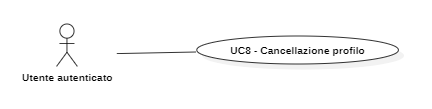
\includegraphics[scale=1]{uc08.png} \end{figure}
\begin{itemize}
\item \textbf{Attore principale:} Utente autenticato;
\item \textbf{Precondizioni:} L'utente è autenticato presso il sistema e sta visualizzando la lista dei suoi profili;
\item \textbf{Postcondizioni:} Il profilo eliminato è rimosso dalla lista dei profili dell'utente;
\item \textbf{Scenario principale:}
\begin{enumerate}
    \item L'utente seleziona l'opzione di eliminazione di un profilo;
    \item Il sistema chiede all'utente di scegliere quale profilo eliminare;
    \item L'utente sceglie il profilo;
    \item L'utente sceglie l'opzione di conferma;
    \item Il sistema comunica all'utente che l'eliminazione del profilo è avvenuta con successo;
    \item L'utente visualizza la lista dei suoi profili dalla quale è stato rimosso il profilo appena creato.
\end{enumerate}
\end{itemize}

\subsubsection{UC9-Selezione profilo cliente}
\begin{figure}[h] 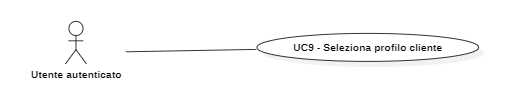
\includegraphics[scale=1]{uc09.png} \end{figure}
\begin{itemize}
\item \textbf{Attore principale:} Utente autenticato;
\item \textbf{Precondizioni:} L'utente è autenticato presso il sistema;
\item \textbf{Postcondizioni:} L'utente visualizza le informazioni relative al profilo cliente selezionato;
\item \textbf{Scenario principale:}
\begin{enumerate}
    \item L'utente sta visualizzando la lista dei suoi profili;
    \item L'utente seleziona un profilo di tipo cliente;
    \item L'utente visualizza la dashboard relativa al profilo selezionato.
\end{enumerate}
\end{itemize}

\pagebreak
\subsubsection{UC10-Selezione profilo ristoratore}
\begin{figure}[h] 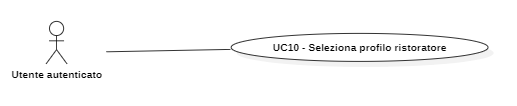
\includegraphics[scale=1]{uc10.png} \end{figure}
\begin{itemize}
\item \textbf{Attore principale:} Utente autenticato;
\item \textbf{Precondizioni:} L'utente è autenticato presso il sistema e possiede un profilo ristoratore;
\item \textbf{Postcondizioni:} L'utente visualizza le informazioni relative al profilo ristoratore selezionato;
\item \textbf{Scenario principale:}
\begin{enumerate}
    \item L'utente sta visualizzando la lista dei suoi profili;
    \item L'utente seleziona un profilo di tipo ristoratore;
    \item L'utente visualizza la dashboard relativa al ristorante del profilo selezionato.
\end{enumerate}
\end{itemize}

\subsubsection{UC11-Modifica profilo}
\begin{figure}[h] 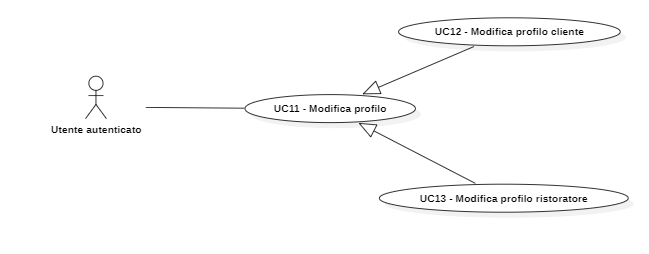
\includegraphics[scale=.7]{uc11.png} \end{figure}
\begin{itemize}
\item \textbf{Attore principale:} Utente autenticato;
\item \textbf{Precondizioni:} L'utente è stato autenticato dal sistema e sta visualizzando la lista dei suoi profili;
\item \textbf{Postcondizioni:} Le modifiche apportate ai dati relativi al profilo sono salvate dal sistema;
\item \textbf{Scenario principale:}
\begin{enumerate}
    \item L'utente seleziona l'opzione di modifica del profilo;
    \item L'utente seleziona il profilo da modificare;
    \item L'utente visualizza i campi-dati modificabili del profilo;
    \item L'utente modifica uno o più dei campi-dati;
    \item L'utente conferma al sistema la o le modifiche effettuate;
    \item Il sistema comunica all'utente che la modifica è avvenuta con successo;
    \item L'utente visualizza la lista dei suoi profili.
\end{enumerate}
    \item \textbf{Specializzazioni:}
        \begin{itemize}
            \item UC12-Modifica profilo cliente;
            \item UC13-Modifica profilo ristoratore.
        \end{itemize}
\end{itemize}

\subsubsection{UC12-Modifica profilo cliente}
\begin{itemize}
\item \textbf{Attore principale:} Utente autenticato / Cliente;
\item \textbf{Precondizioni:} L'utente è stato autenticato dal sistema e sta visualizzando la lista dei suoi profili;
\item \textbf{Postcondizioni:} Le modifiche apportate ai dati relativi al profilo sono salvate dal sistema;
\item \textbf{Scenario principale:}
\begin{enumerate}
    \item L'utente seleziona l'opzione di modifica del profilo;
    \item L'utente seleziona il profilo cliente da modificare;
    \item L'utente visualizza e/o modifica uno o più dei seguenti campi-dati:
        \begin{itemize}
            \item Il nome;
            \item Il cognome;
            \item Lo username;
            \item Le eventuali allergie ed intolleranze da una lista fornita dal sistema.
        \end{itemize}
    \item L'utente modifica uno o più dei campi-dati;
    \item L'utente conferma al sistema la o le modifiche effettuate;
    \item Il sistema comunica all'utente che la modifica è avvenuta con successo;
    \item L'utente visualizza la lista dei suoi profili.
\end{enumerate}
\end{itemize}

\subsubsection{UC13-Modifica profilo ristoratore}
\begin{itemize}
\item \textbf{Attore principale:} Utente autenticato / Ristoratore;
\item \textbf{Precondizioni:} L'utente è stato autenticato dal sistema e sta visualizzando la lista dei suoi profili;
\item \textbf{Postcondizioni:} Le modifiche apportate ai dati relativi al profilo sono salvate dal sistema;
\item \textbf{Scenario principale:}
\begin{enumerate}
    \item L'utente seleziona l'opzione di modifica del profilo;
    \item L'utente seleziona il profilo ristoratore da modificare;
    \item L'utente visualizza e/o modifica uno o più dei seguenti campi-dati:
        \begin{itemize}
            \item Il nome del ristorante;
            \item L'indirizzo;
            \item Giorni di apertura;
            \item Il recapito telefonico;
            \item Il numero di coperti disponibili;
            \item L'elenco delle tipologie di cucine proposte.
        \end{itemize}
    \item L'utente modifica uno o più dei campi-dati;
    \item L'utente conferma al sistema la o le modifiche effettuate;
    \item Il sistema comunica all'utente che la modifica è avvenuta con successo;
    \item L'utente visualizza la lista dei suoi profili.
\end{enumerate}
        \item \textbf{Estensioni:}
        \begin{itemize}
                \item UCE7.1-Campo mancante;
                \item UCE7.2-Recapito telefonico già presente;
                \item UCE7.3-Indirizzo già presente.
        \end{itemize}
\end{itemize}

\subsubsection{UC14-Logout dal profilo}
\begin{figure}[h] 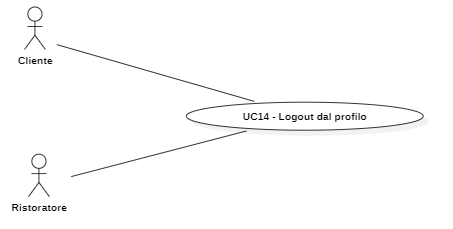
\includegraphics[scale=1]{uc14.png} \end{figure}
\begin{itemize}
\item \textbf{Attore principale:} Cliente / Ristoratore;
\item \textbf{Precondizioni:} L'utente ha selezionato uno dei profili afferenti al suo account;
\item \textbf{Postcondizioni:} L'utente è indirizzato alla pagina di selezione del profilo;
\item \textbf{Scenario principale:}
\begin{enumerate}
    \item L'utente seleziona l'opzione di logout dal profilo precedentemente selezionato;
    \item Il sistema chiede la conferma all'utente della volontà di tornare alla scelta dei profili;
    \item L'utente conferma la scelta;
    \item L'utente visualizza la lista dei profili del suo account, potendone selezionare uno.
\end{enumerate}
\end{itemize}
